\chapter{Segmentation results}
\section{Inclass}\index{Inclass}

\subsection{Image \texttt{10\_27a}}
\begin{figure}[H]
  \begin{subfigure}{.6\textwidth}
    \centering
    \includegraphics[width=.6\linewidth]{/home/rihan/comp510project/output/10_27a.png}
    \caption{Original input \texttt{10\_27a} image}
  \end{subfigure}%
  \begin{subfigure}{.6\textwidth}
    \centering
    \includegraphics[width=.6\linewidth]{/home/rihan/comp510project/output/10_27a_op.jpg}
    \caption{Image after Otsu's Segmentation}
  \end{subfigure}
\end{figure}

\subsection{Image \texttt{10\_27d}}
\begin{figure}[H]
  \begin{subfigure}{.5\textwidth}
    \centering
    \includegraphics[width=.7\linewidth]{/home/rihan/comp510project/output/10_27d.png}
    \caption{Original input \texttt{10\_27d} image}
  \end{subfigure}%
  \begin{subfigure}{.6\textwidth}
    \centering
    \includegraphics[width=.6\linewidth]{/home/rihan/comp510project/output/10_27d_op.jpg}
    \caption{Image after using divide and segment strategy}
  \end{subfigure}
\end{figure}


\pagebreak

\subsection{Image \texttt{son1}}
\begin{figure}[h!]{.6\textwidth}
  \centering
  \includegraphics[width=.7\linewidth]{/home/rihan/comp510project/output/son1.png}
  \caption{Original input \texttt{son1} image}
\end{figure}

\begin{figure}[h!]
  \begin{subfigure}{.6\textwidth}
    \centering
    \includegraphics[width=.7\linewidth]{/home/rihan/comp510project/output/son1_process.png}
    \caption{\texttt{son1 - in process}}
  \end{subfigure}%
  \begin{subfigure}{.6\textwidth}
    \centering
    \includegraphics[width=.7\linewidth]{/home/rihan/comp510project/output/son1_final.png}
    \caption{\texttt{son1} - final outcome}
  \end{subfigure}
\end{figure}

\pagebreak

\subsection{Image \texttt{papir}}

\begin{figure}[h!]
  \begin{subfigure}{.5\textwidth}
    \centering
    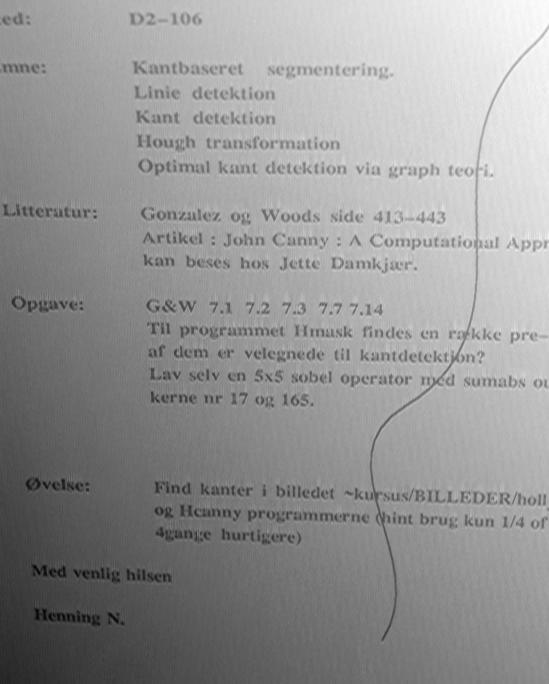
\includegraphics[width=.6\linewidth]{/home/rihan/comp510project/output/papir.jpg}
    \caption{\texttt{papir} - original input image}
  \end{subfigure}%
  \begin{subfigure}{.6\textwidth}
    \centering
    \includegraphics[width=.7\linewidth]{/home/rihan/comp510project/output/papir_2.jpg}
    \caption{\texttt{papir} - after roberts edge detection}
  \end{subfigure}
\end{figure}

\begin{figure}[h!]
  \begin{subfigure}{.6\textwidth}
    \centering
    \includegraphics[width=.6\linewidth]{/home/rihan/comp510project/output/papir_3.jpg}
    \caption{\texttt{papir} - remove small pixels}
  \end{subfigure}%
  \begin{subfigure}{.6\textwidth}
    \centering
    \includegraphics[width=.6\linewidth]{/home/rihan/comp510project/output/papir_dilate.jpg}
    \caption{\texttt{papir} - dilation to thicken hair}
  \end{subfigure}
\end{figure}

\begin{figure}[h!]{.6\textwidth}
  \centering
  \includegraphics[width=.6\linewidth]{/home/rihan/comp510project/output/papir_4.jpg}
  \caption{adaptive threshold on the image to obtain binary image}
\end{figure}
\begin{figure}[h!]{.6\textwidth}
  \centering
  \includegraphics[width=.6\linewidth]{/home/rihan/comp510project/output/papir_5.png}
  \caption{final outcome - addition of binary image \+ dilated image}
\end{figure}

\pagebreak

\section{Extras}\index{Extras}
\subsection{Image \texttt{grp of coins}}
\begin{figure}[h!]
  \centering
  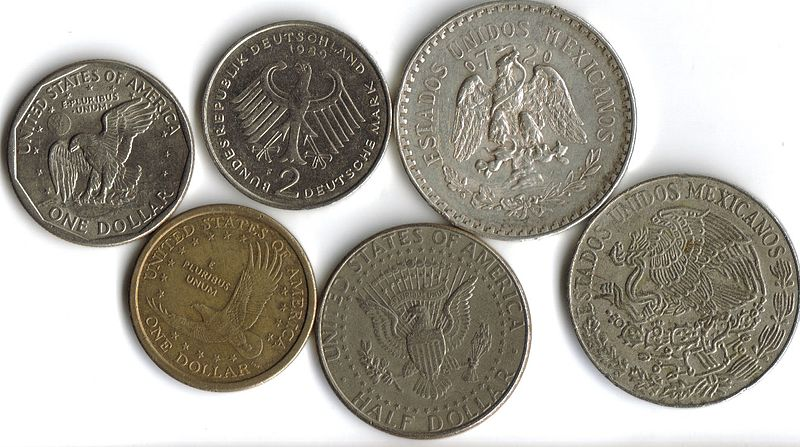
\includegraphics[width=8cm,height=6cm,keepaspectratio]{/home/rihan/comp510project/extras/group_of_coins.jpg}
  \caption{Original input \texttt{grp\_of\_coins} image}
\end{figure}
\begin{figure}[h!]
  \centering
  \includegraphics[width=14cm,height=10cm,keepaspectratio]{/home/rihan/comp510project/output/group_of_coins_inclass.png}
  \caption{segmented image using otsu's method}
\end{figure}

\subsection{Image \texttt{jet\_fighter\_swarm}}
\begin{figure}[h!]
  \centering
  \includegraphics[width=14cm,height=10cm,keepaspectratio]{/home/rihan/comp510project/output/jet.png}
  \caption{segmented image}
\end{figure}

\pagebreak

\subsection{Image - \texttt{grp of coins}(sobel)}
\begin{figure}[h!]
  \centering
  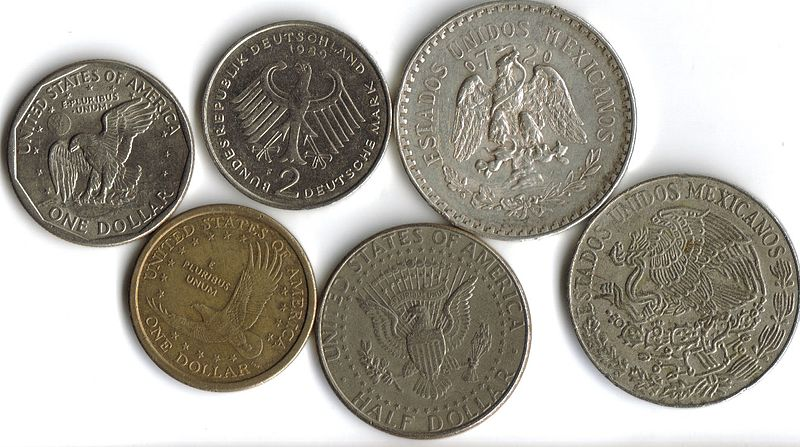
\includegraphics[width=14cm,height=10cm,keepaspectratio]{/home/rihan/comp510project/extras/group_of_coins.jpg}
  \caption{Original input \texttt{grp\_of\_coins} image}
\end{figure}
\begin{figure}[h!]
  \centering
  \includegraphics[width=14cm,height=10cm,keepaspectratio]{/home/rihan/comp510project/output/sobel_grp_of_coins.png}
  \caption{group of coins sobel operator}
\end{figure}

\pagebreak

\subsection{Image - \texttt{another coins}(sobel) }
\begin{figure}[h!]
  \centering
  \includegraphics[width=14cm,height=10cm,keepaspectratio]{/home/rihan/comp510project/extras/another_coins.jpg}
  \caption{Original input \texttt{another\_coins} image}
\end{figure}
\begin{figure}[h!]
  \centering
  \includegraphics[width=14cm,height=10cm,keepaspectratio]{/home/rihan/comp510project/output/sobel_another_coins.png}
  \caption{another coins sobel operator}
\end{figure}

\subsection{Image - \texttt{pillars of hercules}(sobel) }
\begin{figure}[h!]
  \centering
  \includegraphics[width=14cm,height=10cm,keepaspectratio]{/home/rihan/comp510project/extras/hercules_poles.jpg}
  \caption{Original input image}
\end{figure}
\begin{figure}[h!]
  \centering
  \includegraphics[width=14cm,height=10cm,keepaspectratio]{/home/rihan/comp510project/output/sobel_poh.png}
  \caption{outcome using sobel operator}
\end{figure}

\subsection{Image - \texttt{group of coins}(canny) }
\begin{figure}[h!]
  \centering
  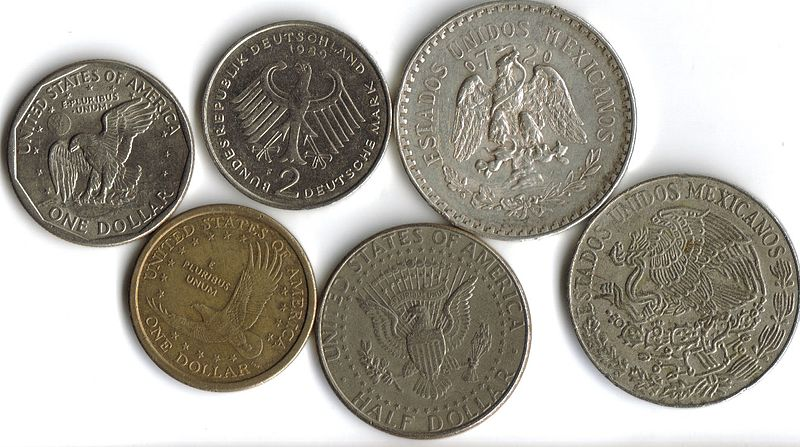
\includegraphics[width=14cm,height=10cm,keepaspectratio]{/home/rihan/comp510project/extras/group_of_coins.jpg}
  \caption{Original input image}
\end{figure}
\begin{figure}[h!]
  \centering
  \includegraphics[width=14cm,height=10cm,keepaspectratio]{/home/rihan/comp510project/output/canny_grp_of_coins.png}
  \caption{outcome using canny edge detector}
\end{figure}

\pagebreak

\subsection{Image - \texttt{another coins}(canny) }
\begin{figure}[h!]
  \centering
  \includegraphics[width=14cm,height=10cm,keepaspectratio]{/home/rihan/comp510project/extras/another_coins.jpg}
  \caption{Original input image}
\end{figure}
\begin{figure}[h!]
  \centering
  \includegraphics[width=14cm,height=10cm,keepaspectratio]{/home/rihan/comp510project/output/canny_another_coins.png}
  \caption{outcome using canny edge detector}
\end{figure}

\subsection{Image - \texttt{pillars of hercules}(canny) }
\begin{figure}[h!]
  \centering
  \includegraphics[width=14cm,height=10cm,keepaspectratio]{/home/rihan/comp510project/extras/hercules_poles.jpg}
  \caption{Original input image}
\end{figure}
\begin{figure}[h!]
  \centering
  \includegraphics[width=14cm,height=10cm,keepaspectratio]{/home/rihan/comp510project/output/canny_poh.png}
  \caption{outcome using canny edge detector}
\end{figure}

\pagebreak
\subsection{Image - \texttt{baby elephant}(morphology) }
\begin{figure}[h!]
  \centering
  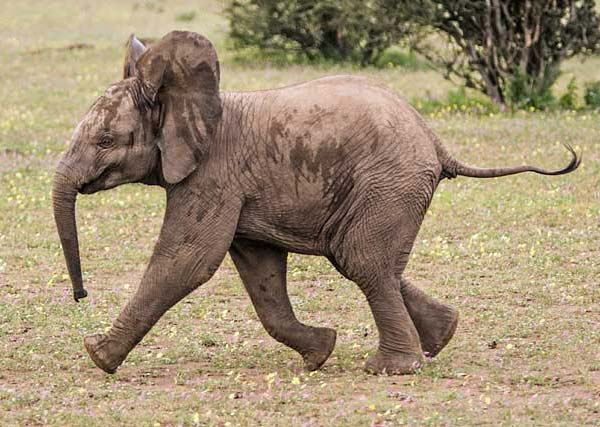
\includegraphics[width=14cm,height=10cm,keepaspectratio]{/home/rihan/comp510project/extras/elephant_identify.jpg}
  \caption{Original input image}
\end{figure}
\begin{figure}[h!]
  \centering
  \includegraphics[width=14cm,height=10cm,keepaspectratio]{/home/rihan/comp510project/output/elph_bg_elm.png}
  \caption{background elimination using berosion}
\end{figure}

\begin{figure}[h!]
  \centering
  \includegraphics[width=14cm,height=10cm,keepaspectratio]{/home/rihan/comp510project/output/elph_body.png}
  \caption{final result, best of our ability}
\end{figure}

\subsection{Image - \texttt{baby elephant}(maximum filter) }
\begin{figure}[h!]
  \centering
  \includegraphics[width=14cm,height=10cm,keepaspectratio]{/home/rihan/comp510project/output/max_grp_of_coins.png}
  \caption{outcome of group of coins image}
\end{figure}

\begin{figure}[h!]
  \centering
  \includegraphics[width=14cm,height=10cm,keepaspectratio]{/home/rihan/comp510project/output/maxf_another_coins.png}
  \caption{outcome of another coins image}
\end{figure}

%%% Local Variables:
%%% mode: latex
%%% TeX-master: t
%%% End:
